\documentclass[a4paper]{article}
\usepackage{iftex}
\ifPDFTeX
  \usepackage{vntex}% pdfLaTeX: gói tiếng Việt của template
\else
  \usepackage{fontspec}% XeLaTeX/LuaLaTeX: dùng Latin Modern (có đủ dấu tiếng Việt)
  \setmainfont{Latin Modern Roman}\setsansfont{Latin Modern Sans}\setmonofont{Latin Modern Mono}
\fi
\usepackage{a4wide,amssymb,epsfig,latexsym,multicol,array,hhline,fancyhdr}
\usepackage{booktabs}
\usepackage{amsmath}
\usepackage{lastpage}
\usepackage{enumerate}
\usepackage{color}
\usepackage{graphicx}
\usepackage{array}
\usepackage{tabularx, caption}
\usepackage{subcaption}
\usepackage{longtable}
\usepackage{multirow}
\usepackage[framemethod=tikz]{mdframed}
\usepackage{rotating}
\usepackage{geometry}
\usepackage{setspace}
\usepackage{tikz}
\usepackage{listings}
\usetikzlibrary{arrows.meta,positioning,shapes.geometric,calc,backgrounds}
\usepackage{hyperref}
\hypersetup{urlcolor=blue,linkcolor=black,citecolor=black,colorlinks=true}

\newtheorem{theorem}{{\bf Định lý}}
\newtheorem{property}{{\bf Tính chất}}
\newtheorem{proposition}{{\bf Mệnh đề}}
\newtheorem{corollary}[proposition]{{\bf Hệ quả}}
\newtheorem{lemma}[proposition]{{\bf Bổ đề}}

%%% ====== THÔNG TIN NHÓM: sửa các dòng màu đỏ [..] trước khi nộp ======
\newcommand{\TODO}[1]{\textcolor{red}{[#1]}}
\newcommand{\GVHD}{Từ Lãng Phiêu}
\newcommand{\st}[1]{\texttt{#1}}
\newcommand{\ra}{\ensuremath{\rightarrow}}

\setlength{\headheight}{40pt}
\pagestyle{fancy}
\fancyhead{}
\fancyhead[L]{
 \begin{tabular}{rl}
    \begin{picture}(25,15)(0,0)
    \put(0,-8){
\includegraphics[width=8mm, height=8mm]{logoITSGUsmall.png}}
   \end{picture}&
	\begin{tabular}{l}
		\textbf{\bf \ttfamily Trường Đại học Sài Gòn}\\
		\textbf{\bf \ttfamily Khoa Công Nghệ Thông Tin}
	\end{tabular}
 \end{tabular}
}
\fancyhead[R]{\begin{tabular}{l}\tiny \bf \\ \tiny \bf \end{tabular}}
\fancyfoot{}
\fancyfoot[L]{\scriptsize \ttfamily Bài tập lớn môn Công nghệ Phần mềm - Học kỳ I, năm học 2026-2027}
\fancyfoot[R]{\scriptsize \ttfamily Trang {\thepage}/\pageref{LastPage}}
\renewcommand{\headrulewidth}{0.3pt}
\renewcommand{\footrulewidth}{0.3pt}

\setcounter{secnumdepth}{4}
\setcounter{tocdepth}{2}
\renewcommand{\contentsname}{Mục lục}
\renewcommand{\refname}{Tài liệu tham khảo}
\renewcommand{\figurename}{Hình}
\renewcommand{\tablename}{Bảng}
\renewcommand{\lstlistingname}{Mã nguồn}

\definecolor{dkgreen}{rgb}{0,0.6,0}
\definecolor{gray}{rgb}{0.5,0.5,0.5}
\definecolor{mauve}{rgb}{0.58,0,0.82}
\definecolor{brew}{rgb}{0.435,0.271,0.153}
\definecolor{okgreen}{rgb}{0.1,0.55,0.3}
\definecolor{warnred}{rgb}{0.75,0.15,0.15}

\lstset{frame=tb, language={}, aboveskip=3mm, belowskip=3mm, showstringspaces=false, columns=flexible,
  basicstyle={\footnotesize\ttfamily}, numbers=left, numberstyle=\tiny\color{gray}, keywordstyle=\color{blue},
  commentstyle=\color{dkgreen}, stringstyle=\color{mauve}, breaklines=true, breakatwhitespace=true, tabsize=2,
  numbersep=5pt, xleftmargin=1.5em}

\renewcommand{\arraystretch}{1.25}
\newcolumntype{L}[1]{>{\raggedright\arraybackslash}p{#1}}
\newcommand{\hl}[1]{\rowcolor{brew!12}#1}
\usepackage{colortbl}


% --- Macro chèn sơ đồ ---
\newcommand{\dfig}[4][width=\textwidth]{\begin{figure}[htbp]\centering\includegraphics[#1,keepaspectratio,width=\textwidth]{diagrams/#2}\caption{#3}\label{#4}\end{figure}}
\newcommand{\sfig}[3]{\begin{sidewaysfigure}\centering\includegraphics[width=0.96\textheight,height=0.78\textwidth,keepaspectratio]{diagrams/#1}\caption{#2}\label{#3}\end{sidewaysfigure}}
\begin{document}

%%%%%%%%%%%%%%%%%%%% TRANG BÌA %%%%%%%%%%%%%%%%%%%%
\begin{titlepage}
\begin{center}
TRƯỜNG ĐẠI HỌC SÀI GÒN \\
KHOA CÔNG NGHỆ THÔNG TIN
\end{center}
\vspace{1cm}
\begin{figure}[h!]
\begin{center}

\includegraphics[width=3cm]{logoITSGU.png}
\end{center}
\end{figure}
\vspace{1cm}
\begin{center}
\begin{tabular}{c}
	\textbf{{\Large CÔNG NGHỆ PHẦN MỀM}}\\
	~~\\
	\hline
	\\
	\textbf{{\Large Bài tập lớn: Quy trình Agile Scrum}}\\
	\\
	\textbf{{\Huge BrewLite}}\\
	\textbf{{\Large Ứng dụng đặt cà phê không dùng tiền mặt}}\\
	\\
	\hline
\end{tabular}
\end{center}
\vspace{2.5cm}
\begin{table}[h]
\begin{tabular}{rrl}
\hspace{5 cm} & GVHD: & \GVHD \\
& SV: & Lâm Sơn Hùng - 3123560031 \\
\end{tabular}
\vspace{1.5 cm}
\end{table}
\begin{center}
{\footnotesize TP. HỒ CHÍ MINH, THÁNG 11/2026}
\end{center}
\end{titlepage}

\thispagestyle{empty}
\newpage
\tableofcontents
\newpage

%%%%%%%%%%%%%%%%%%%% 1. TÓM TẮT %%%%%%%%%%%%%%%%%%%%
\section{Tóm tắt}
BrewLite là ứng dụng web cho phép khách hàng xem menu, chọn đồ uống kèm size/topping, đặt đơn và \textbf{thanh toán không dùng tiền mặt} chỉ trong vài chạm. Nhóm thực hiện theo quy trình \textbf{Agile Scrum} gồm 3 Sprint với 10 hạng mục Product Backlog (mỗi hạng mục 1 điểm), sử dụng công nghệ bắt buộc \textbf{NestJS} (Backend) và \textbf{Next.js} (Frontend), CSDL PostgreSQL.

\begin{itemize}
  \item \textbf{Kết quả:} hoàn thành đủ 10/10 task, đạt Definition of Done (Mục~\ref{sec:dod}). Luồng end-to-end chọn sản phẩm $\to$ giỏ hàng $\to$ đăng nhập $\to$ thanh toán $\to$ xác nhận đơn chạy được từ trình duyệt.
  \item \textbf{Kiểm thử:} 34 test tự động (11 unit + 23 integration trên PostgreSQL thật) đều đạt; ba tiêu chí chấm của Task 10 (chặn chuyển trạng thái sai, idempotent, không bán vượt tồn kho) đều có test chứng minh (Mục~\ref{sec:test}). Thêm 55 kịch bản kiểm thử giao diện (224 điểm kiểm tra) đã phát hiện và sửa 6 lỗi nghiệp vụ (Mục~\ref{sec:uitest}).
  \item \textbf{Bàn giao:} mã nguồn Git, \texttt{docker-compose.yml} chạy cả 3 dịch vụ (frontend, backend, DB), README hướng dẫn chạy (Mục~\ref{sec:handover}).
\end{itemize}

%%%%%%%%%%%%%%%%%%%% 2. SCRUM %%%%%%%%%%%%%%%%%%%%
\section{Quy trình Agile Scrum áp dụng}
\subsection{Vai trò, Sự kiện, Tạo phẩm}
\begin{table}[h!]
\centering
\begin{tabularx}{\textwidth}{|L{3.2cm}|X|}
\hline
\textbf{Nhóm yếu tố} & \textbf{Áp dụng trong BrewLite} \\ \hline
Vai trò (Roles) & \textbf{Product Owner}: Lâm Sơn Hùng --- xác định yêu cầu, sắp xếp ưu tiên Product Backlog, nghiệm thu Increment.\newline
\textbf{Scrum Master}: Lâm Sơn Hùng --- điều phối Daily Scrum, gỡ vướng mắc, đảm bảo quy trình.\newline
\textbf{Development Team}: Lâm Sơn Hùng --- phân tích, thiết kế, lập trình, kiểm thử, bàn giao. Do dự án có một thành viên nên một người kiêm cả ba vai trò; các sự kiện Scrum được thực hiện ở quy mô cá nhân (tự lập kế hoạch, tự cập nhật Burndown, tự review và tự rút kinh nghiệm). \\ \hline
Sự kiện (Events) & Sprint Planning (đầu Sprint, chọn task và ước lượng story point); Daily Scrum (15 phút/ngày, cập nhật Burndown); Sprint Review (demo Increment cho PO); Sprint Retrospective (cuối Sprint). \\ \hline
Tạo phẩm (Artifacts) & Product Backlog (10 task, Mục~\ref{sec:backlog}); Sprint Backlog (task của từng Sprint, Mục~\ref{sec:sprints}); Increment (bản chạy được sau mỗi Sprint, có test và README). \\ \hline
\end{tabularx}
\caption{Vai trò, sự kiện và tạo phẩm Scrum của nhóm}
\end{table}

Hình~\ref{fig:scrum} mô tả chu trình Scrum áp dụng.
\begin{figure}[h!]\centering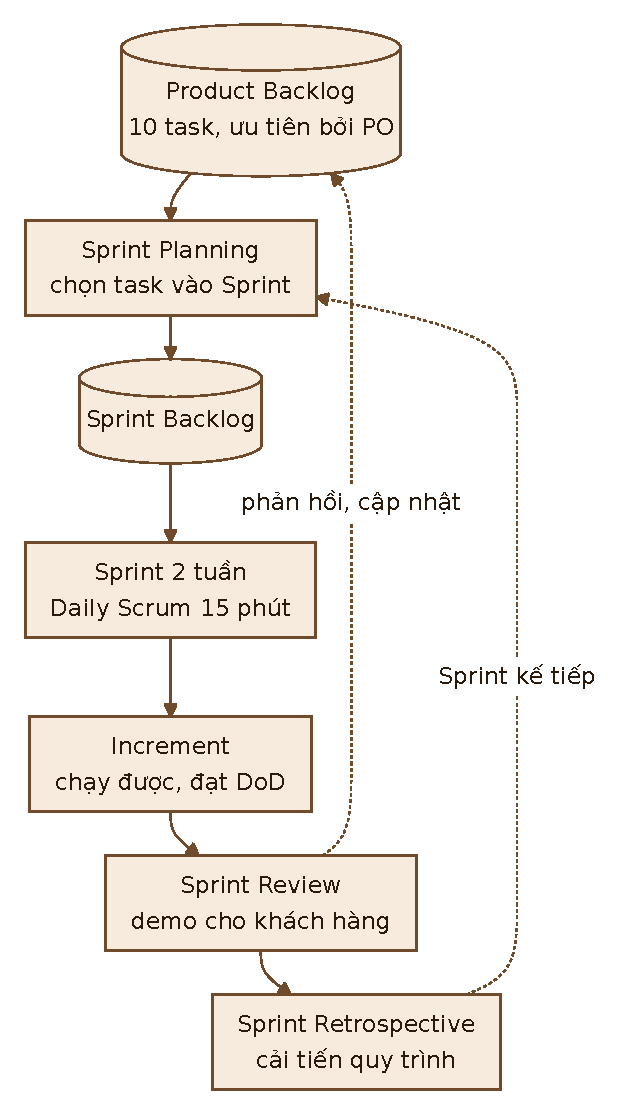
\includegraphics[height=0.42\textheight,keepaspectratio]{diagrams/scrum.pdf}\caption{Chu trình Scrum của dự án}\label{fig:scrum}\end{figure}

\subsection{Kế hoạch 3 Sprint}\label{sec:sprints}
Mỗi Sprint dài 10 ngày liên tục (kể cả cuối tuần); ba Sprint diễn ra từ 12/10/2026 đến 10/11/2026 và Sprint Review/Demo vào 11/11/2026. Story point (SP) là ước lượng tương đối của nhóm; các task được xếp từ dễ đến khó theo Product Backlog.

\begin{table}[h!]
\centering
\begin{tabularx}{\textwidth}{|L{1.8cm}|L{4.6cm}|L{3.4cm}|X|}
\hline
\textbf{Sprint} & \textbf{Mục tiêu (Sprint Goal)} & \textbf{Task} & \textbf{SP} \\ \hline
Sprint 1 \newline 12/10--21/10 & Nền tảng và hiển thị menu: khởi tạo dự án, API và trang Menu, chi tiết sản phẩm & Task 1, 2, 3, 4 & 2+2+3+3 = 10 \\ \hline
Sprint 2 \newline 22/10--31/10 & Giỏ hàng, đặt đơn và đăng nhập: khách có thể đăng nhập và tạo đơn \st{PENDING} & Task 5, 6, 7 & 3+3+3 = 9 \\ \hline
Sprint 3 \newline 01/11--10/11 & Thanh toán, bàn giao và nghiệp vụ nâng cao: thanh toán không tiền mặt, lịch sử đơn, Docker, nghiệp vụ backend & Task 8, 9, 10 & 3+3+8 = 14 \\ \hline
\multicolumn{3}{|r|}{\textbf{Tổng}} & \textbf{33} \\ \hline
\end{tabularx}
\caption{Kế hoạch 3 Sprint}
\end{table}

\begin{figure}[h!]\centering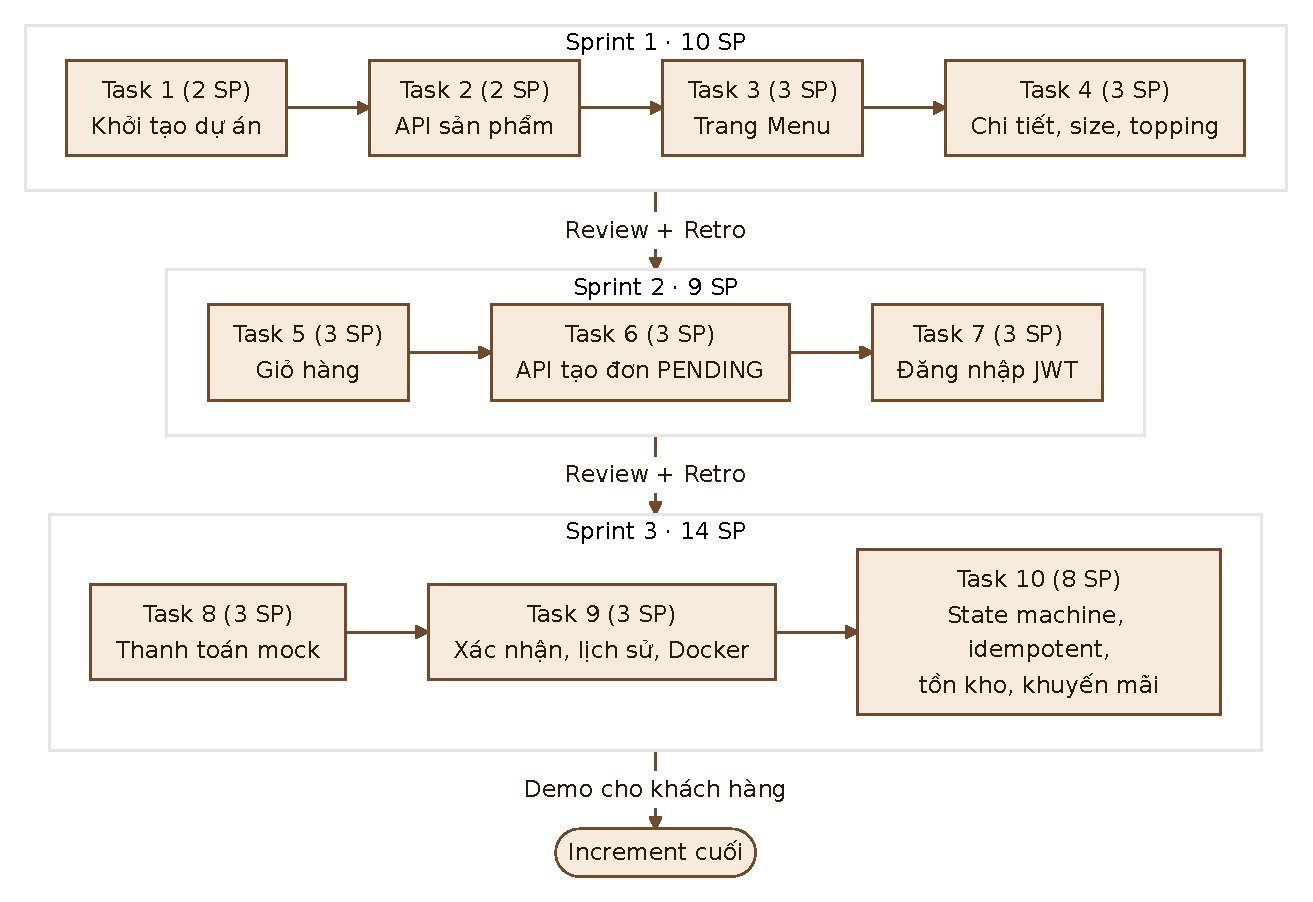
\includegraphics[width=\textwidth,keepaspectratio]{diagrams/roadmap.pdf}\caption{Roadmap: phân bổ 10 task vào 3 Sprint}\label{fig:roadmap}\end{figure}

\subsection{Sprint Burndown chart}
Burndown chart theo dõi khối lượng việc còn lại (story point) giảm dần theo từng ngày. Đường lý tưởng (Ideal) giảm đều; đường thực tế (Actual) phản ánh tiến độ thật. Hình~\ref{fig:burndown} là đường lý tưởng của Sprint 3 (14 SP, 10 ngày) cùng đường thực tế; số điểm còn lại cuối mỗi ngày được ghi ở Bảng~\ref{tab:burndown}.

\begin{figure}[h!]
\centering
\begin{tikzpicture}[x=1.1cm,y=0.33cm]
  \draw[->] (0,0) -- (10.6,0) node[right] {\scriptsize ngày};
  \draw[->] (0,0) -- (0,15.5) node[above] {\scriptsize SP còn lại};
  \foreach \x in {0,...,10} {\draw (\x,0.2) -- (\x,-0.2) node[below] {\scriptsize \x};}
  \foreach \y in {0,2,...,14} {\draw (0.1,\y) -- (-0.1,\y) node[left] {\scriptsize \y}; \draw[gray!30] (0,\y) -- (10,\y);}
  \draw[brew,very thick] (0,14) -- (10,0);
  \node[brew,anchor=west] at (5.2,10.6) {\scriptsize Lý tưởng (Ideal)};
  % TODO-EDIT: sửa toạ độ cho khớp số liệu thực tế (Bảng burndown)
  \draw[red!70,very thick] (0,14)--(1,14)--(2,14)--(3,11)--(4,11)--(5,8)--(6,8)--(7,6)--(8,4)--(9,2)--(10,0);
  \foreach \p in {(0,14),(1,14),(2,14),(3,11),(4,11),(5,8),(6,8),(7,6),(8,4),(9,2),(10,0)} {\fill[red!70] \p circle (1.6pt);}
  \node[red!70,anchor=west,font=\scriptsize] at (6.3,12.2) {Thực tế (Actual)};
\end{tikzpicture}
\caption{Burndown Sprint 3: lý tưởng và thực tế (14 SP / 10 ngày)}\label{fig:burndown}
\end{figure}

\begin{table}[h!]
\centering\small
\begin{tabular}{|l|*{11}{c|}}
\hline
Ngày & 0 & 1 & 2 & 3 & 4 & 5 & 6 & 7 & 8 & 9 & 10 \\ \hline
Ideal (SP) & 14 & 12,6 & 11,2 & 9,8 & 8,4 & 7 & 5,6 & 4,2 & 2,8 & 1,4 & 0 \\ \hline
Actual (SP) & 14 & 14 & 14 & 11 & 11 & 8 & 8 & 6 & 4 & 2 & 0 \\ % TODO-EDIT: số liệu thực tế \hline
\end{tabular}
\caption{Bảng theo dõi Burndown Sprint 3 (số điểm còn lại cuối mỗi ngày)}\label{tab:burndown}
\end{table}

%%%%%%%%%%%%%%%%%%%% 3. SẢN PHẨM %%%%%%%%%%%%%%%%%%%%
\section{Sản phẩm và người dùng}
\subsection{Product Vision}
\begin{quote}\itshape
``BrewLite giúp khách hàng đặt và thanh toán đồ uống không dùng tiền mặt chỉ trong vài chạm, giảm thời gian xếp hàng và nhận đơn nhanh tại quầy.''
\end{quote}

\subsection{Các bên liên quan (Stakeholders)}
\begin{itemize}
  \item \textbf{Khách hàng:} đặt đồ uống, chọn size/topping, thanh toán không tiền mặt, theo dõi trạng thái đơn.
  \item \textbf{Nhân viên quầy/Barista:} tiếp nhận đơn, cập nhật trạng thái pha chế. Ngoài phạm vi MVP, nhóm chỉ cung cấp API \texttt{PATCH /orders/:id/status} (phần mở rộng).
  \item \textbf{Quản lý cửa hàng/Product Owner:} xác định yêu cầu, ưu tiên backlog, nghiệm thu Increment.
  \item \textbf{Giảng viên nghiệm thu:} đánh giá quy trình, sản phẩm và tiêu chí chấp nhận.
  \item \textbf{Nhóm phát triển:} phân tích, thiết kế, lập trình, kiểm thử, bàn giao.
  \item \textbf{Đơn vị thanh toán:} được mô phỏng bằng Mock Payment Gateway (Ví/Thẻ) trong phạm vi bài tập lớn.
\end{itemize}

%%%%%%%%%%%%%%%%%%%% 4. YÊU CẦU %%%%%%%%%%%%%%%%%%%%
\section{Yêu cầu phần mềm}
\subsection{Yêu cầu chức năng (Functional)}
\begin{table}[h!]
\centering
\begin{tabularx}{\textwidth}{|L{1cm}|X|L{2.6cm}|}
\hline
\textbf{Mã} & \textbf{Yêu cầu} & \textbf{Task} \\ \hline
FR1 & Hiển thị danh sách (menu) đồ uống kèm hình, tên, giá. & Task 2, 3 \\ \hline
FR2 & Xem chi tiết sản phẩm, chọn size và topping; giá thay đổi theo tuỳ chọn. & Task 4 \\ \hline
FR3 & Thêm/sửa/xóa sản phẩm trong giỏ hàng; tự tính tổng tiền. & Task 5 \\ \hline
FR4 & Đăng ký / đăng nhập tài khoản (JWT). & Task 7 \\ \hline
FR5 & Tạo đơn hàng và thanh toán không tiền mặt. & Task 6, 8 \\ \hline
FR6 & Hiển thị xác nhận đơn (mã đơn, trạng thái) và lịch sử đơn. & Task 9 \\ \hline
FR7 & Nghiệp vụ nâng cao: state machine, idempotent, tồn kho đồng thời, khuyến mãi/điểm thưởng. & Task 10 \\ \hline
\end{tabularx}
\caption{Yêu cầu chức năng và task tương ứng}
\end{table}

\subsection{Yêu cầu phi chức năng (Non-functional)}
\begin{table}[h!]
\centering
\begin{tabularx}{\textwidth}{|L{3cm}|L{4.2cm}|X|}
\hline
\textbf{Yêu cầu} & \textbf{Cách đáp ứng} & \textbf{Kiểm chứng} \\ \hline
Thời gian phản hồi API $<$ 500\,ms với dữ liệu mẫu & Truy vấn đơn giản, kết nối pool tối đa 20, không N+1 & Đo 30 lần mỗi endpoint (Bảng~\ref{tab:perf}): tất cả $<$ 80\,ms \\ \hline
Bảo mật: băm mật khẩu, JWT, validate đầu vào & bcrypt (cost 10), Passport-JWT, \texttt{ValidationPipe} (whitelist, forbidNonWhitelisted); giá luôn tính lại ở server & Test \texttt{passwordHash} bắt đầu bằng \texttt{\$2}; 401 khi thiếu/sai token; 400 khi dữ liệu sai hoặc có trường lạ \\ \hline
Chạy trên trình duyệt web & Next.js + TailwindCSS, bố cục responsive & Kiểm thử UI bằng Chromium (Playwright) \\ \hline
\end{tabularx}
\caption{Yêu cầu phi chức năng}
\end{table}

\begin{table}[h!]
\centering\small
\begin{tabular}{|l|r|r|r|}
\hline
\textbf{Endpoint (30 lần, máy phát triển)} & \textbf{Trung bình} & \textbf{P95} & \textbf{Lớn nhất} \\ \hline
\texttt{GET /products} & 1,9 ms & 3,6 ms & 4,8 ms \\ \hline
\texttt{GET /products/:id} & 1,9 ms & 3,6 ms & 4,9 ms \\ \hline
\texttt{POST /auth/login} (bcrypt) & 68,2 ms & 75,5 ms & 78,2 ms \\ \hline
\texttt{POST /orders} & 8,5 ms & 11,7 ms & 16,2 ms \\ \hline
\texttt{POST /payments} & 7,5 ms & 10,9 ms & 12,0 ms \\ \hline
\texttt{GET /orders/me} & 2,7 ms & 3,9 ms & 7,1 ms \\ \hline
\end{tabular}
\caption{Thời gian phản hồi API (máy cục bộ, PostgreSQL cục bộ, dữ liệu mẫu)}\label{tab:perf}
\end{table}

\subsection{User Story}
\begin{longtable}{|L{1.4cm}|L{5.4cm}|L{6.3cm}|}
\hline
\textbf{Mã} & \textbf{User Story} & \textbf{Tiêu chí chấp nhận (rút gọn)} \\ \hline
\endhead
US-01 & Là khách hàng, tôi muốn xem menu có hình, tên, giá để chọn đồ uống. & Lưới sản phẩm; có trạng thái loading, rỗng, lỗi + thử lại; sản phẩm hết hàng hiển thị ``Hết hàng''. \\ \hline
US-02 & Là khách hàng, tôi muốn chọn size và topping để đồ uống đúng ý. & Size S/M/L, 4 topping; giá cập nhật ngay; server tính lại giá khi tạo đơn. \\ \hline
US-03 & Là khách hàng, tôi muốn quản lý giỏ hàng để kiểm soát tổng tiền. & Thêm/sửa số lượng/xóa; gộp dòng trùng; tổng tiền và badge số lượng tự cập nhật; giữ giỏ khi tải lại trang. \\ \hline
US-04 & Là khách hàng, tôi muốn đăng ký và đăng nhập để đặt đơn. & Đăng ký/đăng nhập trả JWT; mật khẩu băm; chưa đăng nhập bấm thanh toán thì chuyển tới \texttt{/login}. \\ \hline
US-05 & \textbf{Thanh toán không tiền mặt.} Là khách hàng, tôi muốn thanh toán bằng ví điện tử/thẻ để không cần mang tiền mặt. & Giỏ có $\ge$ 1 sản phẩm thì nút ``Thanh toán'' hiển thị tổng tiền; chọn Ví/Thẻ và xác nhận $\Rightarrow$ đơn \st{PAID}; lỗi $\Rightarrow$ \st{PAYMENT\_FAILED} và giỏ hàng giữ nguyên; thành công hiển thị mã đơn. \\ \hline
US-06 & Là khách hàng, tôi muốn xem xác nhận và lịch sử đơn để theo dõi. & Màn hình xác nhận (mã đơn, trạng thái, ``Mời tới quầy lấy nước''); \texttt{GET /orders/me} chỉ trả đơn của mình. \\ \hline
US-07 & Là khách hàng, tôi muốn bấm thanh toán nhiều lần/mất mạng mà không bị trừ tiền hai lần. & Cùng \texttt{Idempotency-Key} chỉ tạo 1 đơn/1 giao dịch; trả lại kết quả cũ. \\ \hline
US-08 & Là cửa hàng, tôi muốn hệ thống không bán vượt số lượng còn lại. & Đặt đồng thời không làm tồn kho âm; thiếu hàng trả \texttt{409 OUT\_OF\_STOCK}. \\ \hline
US-09 & Là khách hàng, tôi muốn dùng mã giảm giá và tích điểm. & Mã hợp lệ giảm giá đúng; điểm cộng 1 lần sau khi \st{PAID}. \\ \hline
\caption{Các User Story của BrewLite}
\end{longtable}

%%%%%%%%%%%%%%%%%%%% 5. LUỒNG NGHIỆP VỤ %%%%%%%%%%%%%%%%%%%%
\section{Luồng nghiệp vụ: từ chọn sản phẩm đến thanh toán}
\begin{figure}[h!]
\centering
\begin{tikzpicture}[node distance=5mm and 7mm, every node/.style={font=\scriptsize},
  box/.style={draw=brew,rounded corners,fill=brew!8,minimum height=9mm,text width=2.7cm,align=center},
  bad/.style={draw=warnred,rounded corners,fill=red!6,minimum height=9mm,text width=3.6cm,align=center},
  ok/.style={draw=okgreen,rounded corners,fill=green!8,minimum height=9mm,text width=2.7cm,align=center},
  arr/.style={-{Stealth},thick,brew}]
  \node[box] (a) {Mở app};
  \node[box,right=of a] (b) {Xem menu};
  \node[box,right=of b] (c) {Chọn sản phẩm (size, topping)};
  \node[box,below=9mm of c] (d) {Thêm vào giỏ hàng};
  \node[box,left=of d] (e) {Xem giỏ và tổng tiền};
  \node[box,left=of e] (f) {Đăng nhập (nếu chưa)};
  \node[box,below=9mm of f] (g) {Thanh toán không tiền mặt};
  \node[ok,right=of g] (h) {Xác nhận đơn (mã đơn, PAID)};
  \node[ok,right=of h] (i) {Nhận đồ uống};
  \node[bad,below=20mm of g] (x) {Lỗi / hủy: PAYMENT\_FAILED, giữ giỏ};
  \draw[arr] (a)--(b); \draw[arr] (b)--(c); \draw[arr] (c)--(d); \draw[arr] (d)--(e);
  \draw[arr] (e)--(f); \draw[arr] (f)--(g); \draw[arr] (g)--(h); \draw[arr] (h)--(i);
  \draw[arr,warnred] ([xshift=-4mm]g.south) -- node[left,font=\scriptsize,warnred] {lỗi} ([xshift=-4mm]x.north);
  \draw[arr,warnred] ([xshift=4mm]x.north) -- node[right,font=\scriptsize,warnred] {thử lại} ([xshift=4mm]g.south);
  \draw[arr,dashed] (d.east) -- ++(6mm,0) |- (c.east) node[pos=.25,right] {mua thêm};
\end{tikzpicture}
\caption{Luồng nghiệp vụ chính (happy path) và nhánh lỗi của MVP}\label{fig:flow}
\end{figure}

Luồng chi tiết giữa giao diện và API:
\begin{enumerate}
  \item Giao diện gọi \texttt{GET /products} và \texttt{GET /products/:id} để hiển thị menu và tuỳ chọn.
  \item Giỏ hàng lưu ở trạng thái client (Zustand, lưu \texttt{localStorage}); chỉ khi thanh toán mới gọi API.
  \item Khách bấm ``Xác nhận thanh toán'': giao diện gọi \texttt{POST /orders} (kèm \texttt{Idempotency-Key}) để tạo đơn \st{PENDING} và giữ kho, rồi \texttt{POST /payments} (kèm \texttt{Idempotency-Key} khác).
  \item Thành công: đơn \st{PAID}, cộng điểm thưởng, xóa giỏ, chuyển tới màn hình xác nhận. Lỗi (HTTP 402): đơn \st{PAYMENT\_FAILED}, giỏ được giữ, khách thử lại bằng key mới trên cùng đơn.
\end{enumerate}

%%%%%%%%%%%%%%%%%%%% 6. KIẾN TRÚC %%%%%%%%%%%%%%%%%%%%
\section{Kiến trúc và công nghệ}
\subsection{Kiến trúc tổng thể}
\begin{figure}[h!]
\centering
\begin{tikzpicture}[every node/.style={font=\scriptsize},
  b/.style={draw=brew,rounded corners,fill=brew!8,minimum height=11mm,text width=2.7cm,align=center},
  arr/.style={-{Stealth},thick,brew}]
  \node[b] (fe) {\textbf{Next.js}\\Frontend SSR/CSR\\cổng 3000};
  \node[b,right=18mm of fe] (be) {\textbf{NestJS}\\REST API\\cổng 3001};
  \node[b,right=18mm of be] (db) {\textbf{PostgreSQL}\\cổng 5432};
  \node[b,below=10mm of be] (pg) {Mock Payment Gateway};
  \draw[arr] (fe) -- node[above] {REST/JSON} node[below] {JWT} (be);
  \draw[arr] (be) -- node[above] {TypeORM} (db);
  \draw[arr] (be) -- node[right] {thanh toán} (pg);
\end{tikzpicture}
\caption{Frontend gọi REST API của backend; backend dùng một CSDL và cổng thanh toán giả lập}\label{fig:arch}
\end{figure}

\begin{table}[h!]
\centering
\begin{tabularx}{\textwidth}{|L{3cm}|X|}
\hline
\textbf{Thành phần} & \textbf{Công nghệ} \\ \hline
Frontend & Next.js 14 (App Router, React, TypeScript), TailwindCSS, Zustand (giỏ hàng, phiên đăng nhập) \\ \hline
Backend & NestJS 10 (TypeScript), REST, class-validator, JWT (Passport), bcrypt \\ \hline
CSDL & PostgreSQL 16 + TypeORM (entity, transaction, optimistic locking bằng \texttt{@VersionColumn}) \\ \hline
Thanh toán & Mock Payment Service (mô phỏng Momo/VNPay/Stripe) \\ \hline
Kiểm thử & Jest, ts-jest, supertest (integration trên PostgreSQL thật), Playwright (UI) \\ \hline
DevOps & Docker Compose (db + backend + frontend), Git, README bàn giao \\ \hline
\end{tabularx}
\caption{Công nghệ sử dụng}
\end{table}

\subsection{Tổ chức mã nguồn backend}
Backend chia module theo nghiệp vụ: \texttt{auth} (đăng ký, đăng nhập, guard JWT và phân quyền), \texttt{products}, \texttt{orders} (tạo đơn, state machine, tồn kho), \texttt{payments} (thanh toán idempotent, cổng giả lập), \texttt{promotions} (mã giảm giá, điểm thưởng), \texttt{seed} (dữ liệu mẫu). Các hàm nghiệp vụ thuần (tính giá, tính giảm giá, state machine) được tách riêng để kiểm thử đơn vị.

\subsection{Mô hình dữ liệu}
Mô hình dữ liệu gồm 6 bảng (mở rộng từ 5 thực thể tối thiểu của đề: thêm \texttt{coupons} và các cột phục vụ Task 10). Sơ đồ ERD đầy đủ ở Hình~\ref{fig:erd} (Mục~\ref{sec:design}).

%%%%%%%%%%%%%%%%%%%% PHÂN TÍCH & THIẾT KẾ (SƠ ĐỒ) %%%%%%%%%%%%%%%%%%%%
\section{Phân tích và thiết kế hệ thống bằng sơ đồ}\label{sec:design}
Chương này trình bày toàn bộ bộ sơ đồ phân tích và thiết kế của BrewLite theo ngôn ngữ UML và các sơ đồ dòng dữ liệu. Mọi sơ đồ được vẽ từ mã nguồn văn bản (Mermaid và Graphviz, thư mục \texttt{report/diagrams/}) và đối chiếu trực tiếp với mã nguồn đã cài đặt, nên có thể sinh lại khi mã thay đổi. Bảng~\ref{tab:diagramindex} liệt kê các loại sơ đồ và mục đích của từng loại.

\begin{table}[h!]
\centering\small
\begin{tabularx}{\textwidth}{|L{1.0cm}|L{4.0cm}|X|L{1.7cm}|}
\hline
\textbf{STT} & \textbf{Loại sơ đồ} & \textbf{Mục đích trong BrewLite} & \textbf{Hình} \\ \hline
1 & Use Case & Tác nhân, chức năng và quan hệ include/extend của hệ thống & \ref{fig:usecase} \\ \hline
2 & Dòng dữ liệu (DFD) mức 0 và mức 1 & Dữ liệu vào/ra hệ thống và 6 tiến trình chính & \ref{fig:dfd0}, \ref{fig:dfd1} \\ \hline
3 & Hoạt động (Activity) & Quy trình từ chọn món đến tạo đơn, và quy trình thanh toán idempotent & \ref{fig:actA}, \ref{fig:actB} \\ \hline
4 & Tuần tự (Sequence) & 5 kịch bản: xác thực, tạo đơn, thanh toán, hủy/cập nhật trạng thái, tranh chấp tồn kho & \ref{fig:seqauth}--\ref{fig:seqrace} \\ \hline
5 & Lớp (Class) & Thực thể, dịch vụ, controller, guard và quan hệ phụ thuộc phía backend & \ref{fig:class} \\ \hline
6 & Thực thể liên kết (ERD) & Lược đồ CSDL PostgreSQL: khóa, ràng buộc UNIQUE, lực lượng quan hệ & \ref{fig:erd} \\ \hline
7 & Máy trạng thái (State) & Vòng đời đơn hàng và vòng đời xử lý một Idempotency-Key & \ref{fig:stateorder}, \ref{fig:statepay} \\ \hline
8 & Thành phần (Component) & Thành phần frontend, backend, ORM, CSDL và giao tiếp giữa chúng & \ref{fig:component} \\ \hline
9 & Gói / Module (Package) & Phụ thuộc giữa các module NestJS & \ref{fig:package} \\ \hline
10 & Triển khai (Deployment) & 3 container Docker Compose, cổng, volume, biến môi trường & \ref{fig:deployment} \\ \hline
11 & Điều hướng giao diện (Sitemap/Navigation) & Các trang Next.js, điều kiện chuyển trang và bảo vệ đăng nhập & \ref{fig:sitemap} \\ \hline
12 & Quy trình Scrum và Roadmap Sprint & Chu trình Scrum và phân bổ 10 task vào 3 Sprint & \ref{fig:scrum}, \ref{fig:roadmap} \\ \hline
13 & Burndown, Wireframe & Theo dõi tiến độ Sprint 3 (Hình~\ref{fig:burndown}); giao diện MVP (Mục~\ref{sec:ui}) & --- \\ \hline
\end{tabularx}
\caption{Danh mục các loại sơ đồ trong báo cáo}\label{tab:diagramindex}
\end{table}

\subsection{Sơ đồ Use Case}
Hệ thống có hai tác nhân người dùng là \textbf{Khách hàng} và \textbf{Nhân viên/Barista}, cùng một tác nhân hệ thống là \textbf{Cổng thanh toán} (giả lập). Hình~\ref{fig:usecase} mô tả 13 use case; Bảng~\ref{tab:ucspec} đặc tả hai use case trọng tâm.

\dfig[height=0.84\textheight]{usecase.pdf}{Sơ đồ Use Case của BrewLite}{fig:usecase}

\begin{table}[h!]
\centering\small
\begin{tabularx}{\textwidth}{|L{2.9cm}|X|}
\hline
\multicolumn{2}{|l|}{\textbf{UC5 -- Đặt đơn (tạo đơn PENDING)}} \\ \hline
Tác nhân & Khách hàng \\ \hline
Tiền điều kiện & Đã đăng nhập (JWT hợp lệ); giỏ hàng có ít nhất 1 dòng. \\ \hline
Luồng chính & (1) Khách chọn phương thức và (tuỳ chọn) nhập mã giảm giá; (2) frontend gửi \texttt{POST /orders} kèm \texttt{Idempotency-Key}; (3) server kiểm tra dữ liệu, tự tính đơn giá và tiền giảm; (4) trừ kho bằng optimistic locking; (5) lưu đơn \texttt{PENDING} và trả mã đơn. \\ \hline
Luồng thay thế & 3a. Dữ liệu sai (giỏ rỗng, size/topping không có, số lượng không hợp lệ): 400. 3b. Mã giảm giá sai/hết hạn/chưa đủ giá trị tối thiểu: 400. 4a. Không đủ hàng: 409 \texttt{OUT\_OF\_STOCK}, kho không đổi. 2a. Gửi lại cùng key: trả đơn cũ (200), không tạo đơn mới. \\ \hline
Hậu điều kiện & Đơn \texttt{PENDING} được lưu; tồn kho đã giảm đúng số lượng; hoặc không có thay đổi nào nếu lỗi (rollback). \\ \hline
\multicolumn{2}{|l|}{\textbf{UC6 -- Thanh toán không tiền mặt}} \\ \hline
Tác nhân & Khách hàng; Cổng thanh toán (mock) \\ \hline
Tiền điều kiện & Đơn của chính khách, ở trạng thái \texttt{PENDING} hoặc \texttt{PAYMENT\_FAILED}. \\ \hline
Luồng chính & (1) Gửi \texttt{POST /payments} với \texttt{Idempotency-Key}; (2) server khóa dòng đơn; (3) gọi cổng thanh toán; (4) thành công: đơn \texttt{PAID}, cộng điểm thưởng đúng 1 lần, lưu payment \texttt{SUCCESS}; (5) frontend xóa giỏ và mở màn hình xác nhận. \\ \hline
Luồng thay thế & 1a. Thiếu key: 400. 1b. Key đã xử lý: trả lại kết quả cũ, không trừ tiền lần hai. 1c. Key đã dùng cho đơn khác: 409. 2a. Đơn đã \texttt{PAID}/\texttt{CANCELLED}...: 409 \texttt{ORDER\_NOT\_PAYABLE}. 4a. Cổng từ chối: đơn \texttt{PAYMENT\_FAILED}, trả 402, giữ nguyên giỏ, cho phép thử lại bằng key mới. \\ \hline
Hậu điều kiện & Mỗi Idempotency-Key tương ứng tối đa 1 giao dịch; trạng thái đơn khớp kết quả thanh toán. \\ \hline
\end{tabularx}
\caption{Đặc tả use case UC5 và UC6}\label{tab:ucspec}
\end{table}

\subsection{Sơ đồ dòng dữ liệu (DFD)}
DFD mức 0 (Hình~\ref{fig:dfd0}) coi hệ thống là một tiến trình duy nhất và cho thấy các luồng dữ liệu với ba tác nhân ngoài. DFD mức 1 (Hình~\ref{fig:dfd1}) phân rã thành 6 tiến trình và 5 kho dữ liệu tương ứng với các bảng CSDL.

\dfig[width=\textwidth]{dfd0.pdf}{DFD mức 0 (sơ đồ ngữ cảnh)}{fig:dfd0}
\dfig[width=\textwidth]{dfd1.pdf}{DFD mức 1: phân rã hệ thống thành 6 tiến trình và 5 kho dữ liệu}{fig:dfd1}

\subsection{Sơ đồ hoạt động (Activity)}
Hình~\ref{fig:actA} mô tả hoạt động của khách hàng và hệ thống từ lúc chọn món đến khi tạo đơn \texttt{PENDING}. Hình~\ref{fig:actB} tiếp nối với quy trình thanh toán idempotent và các nhánh lỗi/thử lại/hủy. Màu sắc: nâu là khách hàng, xanh dương là frontend, xanh lá là backend, xám là cổng thanh toán, đỏ là lỗi.

\dfig[height=0.78\textheight]{activity-a.pdf}{Sơ đồ hoạt động (1): từ chọn món đến tạo đơn}{fig:actA}
\dfig[height=0.78\textheight]{activity-b.pdf}{Sơ đồ hoạt động (2): thanh toán idempotent, thử lại và hủy đơn}{fig:actB}

\subsection{Sơ đồ tuần tự (Sequence)}
Năm sơ đồ tuần tự dưới đây bám sát mã nguồn (tên controller, service, câu lệnh SQL chính). Hình~\ref{fig:seqauth} là đăng ký/đăng nhập và xác thực JWT; Hình~\ref{fig:seqorder} là tạo đơn với kiểm tra Idempotency-Key và trừ kho; Hình~\ref{fig:seqpay} là thanh toán idempotent có khóa dòng; Hình~\ref{fig:seqcancel} là hủy đơn (hoàn kho) và nhân viên cập nhật trạng thái; Hình~\ref{fig:seqrace} minh họa cơ chế optimistic locking khi hai khách tranh sản phẩm cuối cùng.

\dfig[height=0.86\textheight]{seq-auth.pdf}{Sequence: đăng ký, đăng nhập và xác thực JWT}{fig:seqauth}
\dfig[height=0.86\textheight]{seq-order.pdf}{Sequence: tạo đơn (validate, tính giá, giảm giá, trừ kho optimistic lock)}{fig:seqorder}
\dfig[height=0.86\textheight]{seq-pay.pdf}{Sequence: thanh toán idempotent (khóa dòng đơn, ràng buộc UNIQUE)}{fig:seqpay}
\dfig[height=0.86\textheight]{seq-cancel.pdf}{Sequence: khách hủy đơn (hoàn kho) và nhân viên cập nhật trạng thái}{fig:seqcancel}
\dfig[height=0.7\textheight]{seq-race.pdf}{Sequence: hai khách tranh sản phẩm cuối cùng (optimistic locking)}{fig:seqrace}

\subsection{Sơ đồ lớp (Class)}
Hình~\ref{fig:class} gồm sáu thực thể (kiểu \texttt{@Entity} của TypeORM), kiểu liệt kê \texttt{OrderStatus}, các service chứa nghiệp vụ, controller và guard. \texttt{Order} và \texttt{OrderItem} có quan hệ hợp thành (composition); \texttt{OrderItem} lưu \texttt{productName} và \texttt{unitPrice} tại thời điểm mua để lịch sử không bị ảnh hưởng khi menu đổi.

\dfig[height=0.8\textheight]{class-domain.pdf}{Sơ đồ lớp (1): mô hình miền (thực thể và quan hệ)}{fig:class}
\dfig[width=\textwidth]{class-service.pdf}{Sơ đồ lớp (2): controller, service, guard và phụ thuộc}{fig:class2}

\subsection{Sơ đồ thực thể liên kết (ERD)}
Hình~\ref{fig:erd} là lược đồ quan hệ trên PostgreSQL. Các ràng buộc quan trọng: \texttt{users.email} UNIQUE; \texttt{payments.idempotencyKey} UNIQUE (nền tảng của thanh toán idempotent); \texttt{(orders.userId, orders.idempotencyKey)} UNIQUE (chống tạo đơn trùng); cột \texttt{products.version} phục vụ optimistic locking.

\dfig[height=0.72\textheight]{erd.pdf}{Sơ đồ ERD (ký hiệu chân chim)}{fig:erd}

\subsection{Sơ đồ máy trạng thái (State Machine)}
Vòng đời đơn hàng được cài đặt bởi bảng chuyển tiếp trong \texttt{order-status.ts} và được kiểm chứng đủ 49 cặp trạng thái (Mục~\ref{sec:task10}). Hình~\ref{fig:stateorder} là sơ đồ UML tương đương với Hình~\ref{fig:fsm}. Hình~\ref{fig:statepay} mô tả vòng đời xử lý một Idempotency-Key trong \texttt{PaymentsService}.

\dfig[height=0.46\textheight]{state-order.pdf}{State machine của đơn hàng (UML)}{fig:stateorder}
\dfig[height=0.5\textheight]{state-payment.pdf}{State machine xử lý một Idempotency-Key thanh toán}{fig:statepay}

\subsection{Sơ đồ thành phần, gói và triển khai}
Sơ đồ thành phần (Hình~\ref{fig:component}) cho thấy frontend chỉ giao tiếp với backend qua REST/JSON kèm JWT, và mọi truy cập CSDL đi qua TypeORM. Sơ đồ gói (Hình~\ref{fig:package}) cho thấy \texttt{payments} phụ thuộc \texttt{orders}, \texttt{orders} phụ thuộc \texttt{promotions}; mọi module dùng chung lớp \texttt{entities}. Sơ đồ triển khai (Hình~\ref{fig:deployment}) khớp với \texttt{docker-compose.yml}.

\dfig[height=0.82\textheight]{component.pdf}{Sơ đồ thành phần (Component)}{fig:component}
\dfig[width=\textwidth]{package.pdf}{Sơ đồ gói / phụ thuộc module backend}{fig:package}
\dfig[width=\textwidth]{deployment.pdf}{Sơ đồ triển khai (Deployment) với Docker Compose}{fig:deployment}

\subsection{Sơ đồ điều hướng giao diện}
Hình~\ref{fig:sitemap} cho thấy các trang của frontend và điều kiện chuyển trang; trang \texttt{/checkout} và \texttt{/orders} yêu cầu đăng nhập (chuyển sang \texttt{/login?next=...} rồi quay lại). Giao diện từng màn hình xem Mục~\ref{sec:ui}.

\dfig[height=0.62\textheight]{sitemap.pdf}{Sơ đồ điều hướng các trang Next.js}{fig:sitemap}

%%%%%%%%%%%%%%%%%%%% GIAO DIỆN %%%%%%%%%%%%%%%%%%%%
\section{Giao diện MVP}\label{sec:ui}
Giao diện bám sát 5 màn hình wireframe của đề: (1) Menu, (2) Chi tiết, (3) Giỏ hàng, (4) Thanh toán, (5) Xác nhận; bổ sung màn hình thanh toán lỗi và lịch sử đơn. Ảnh chụp từ bản chạy thật.

\begin{figure}[h!]
\centering
\begin{subfigure}{0.49\textwidth}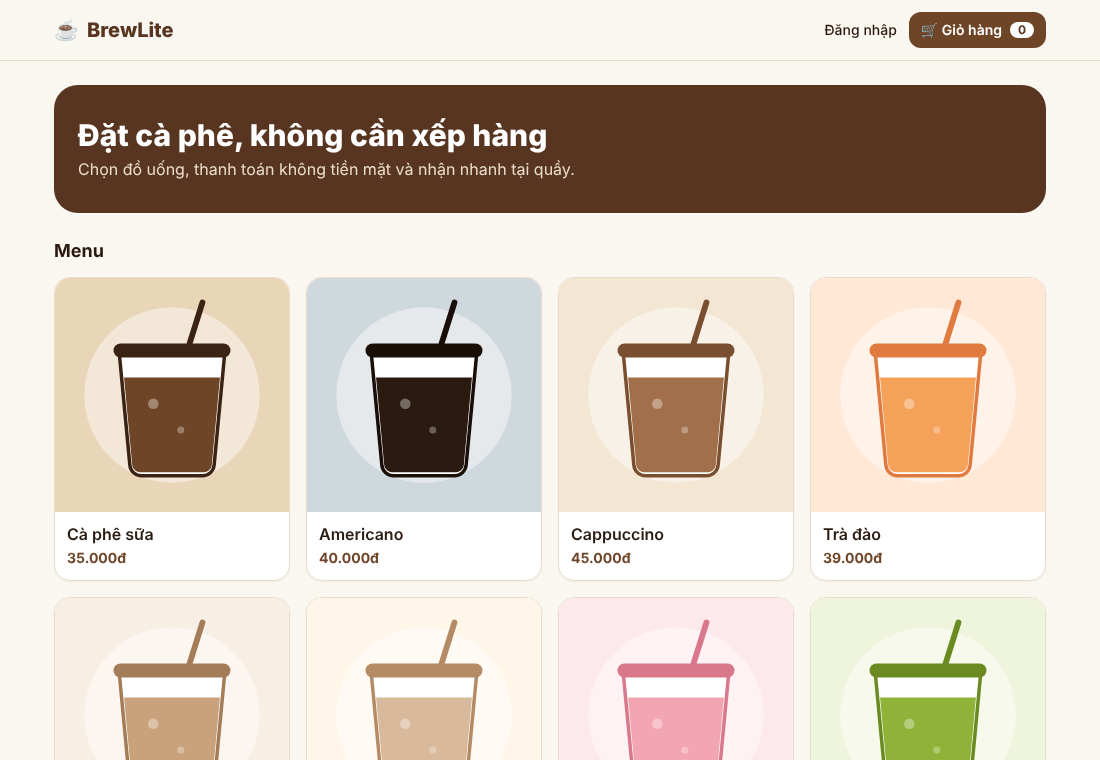
\includegraphics[width=\textwidth]{shots/1-menu.png}\caption{(1) Menu}\end{subfigure}\hfill
\begin{subfigure}{0.49\textwidth}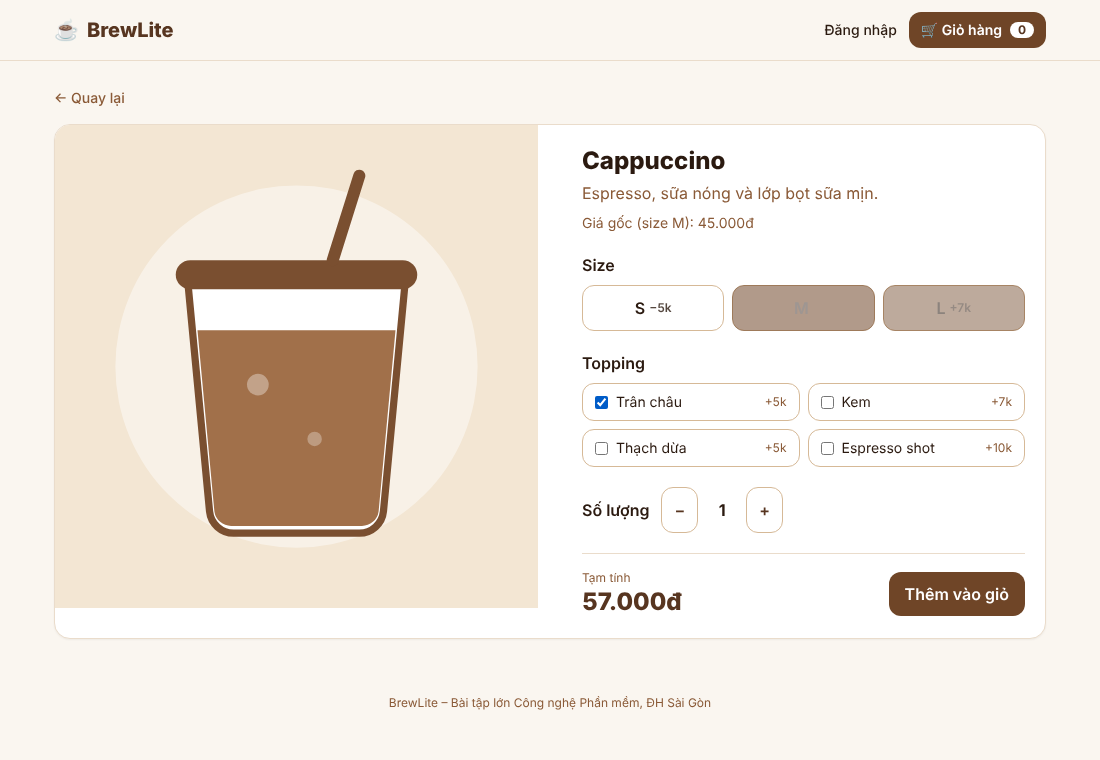
\includegraphics[width=\textwidth]{shots/2-detail.png}\caption{(2) Chi tiết, chọn size/topping}\end{subfigure}
\caption{Màn hình Menu và Chi tiết sản phẩm}
\end{figure}

\begin{figure}[h!]
\centering
\begin{subfigure}{0.49\textwidth}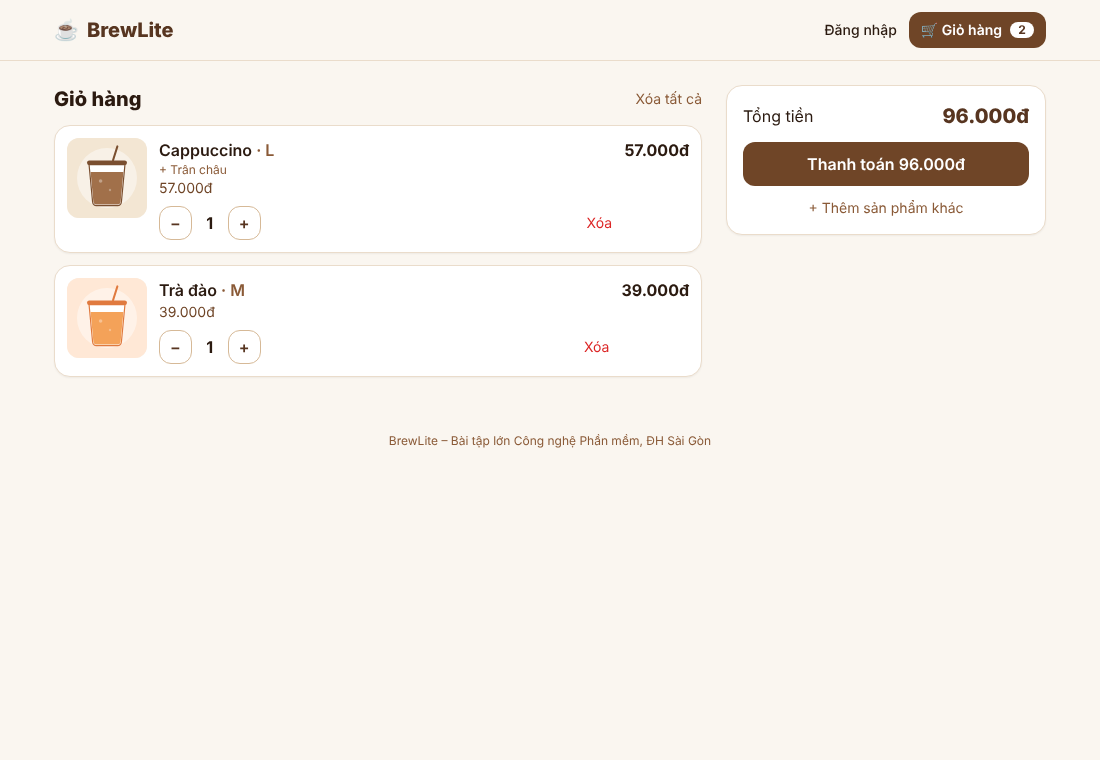
\includegraphics[width=\textwidth]{shots/3-cart.png}\caption{(3) Giỏ hàng}\end{subfigure}\hfill
\begin{subfigure}{0.49\textwidth}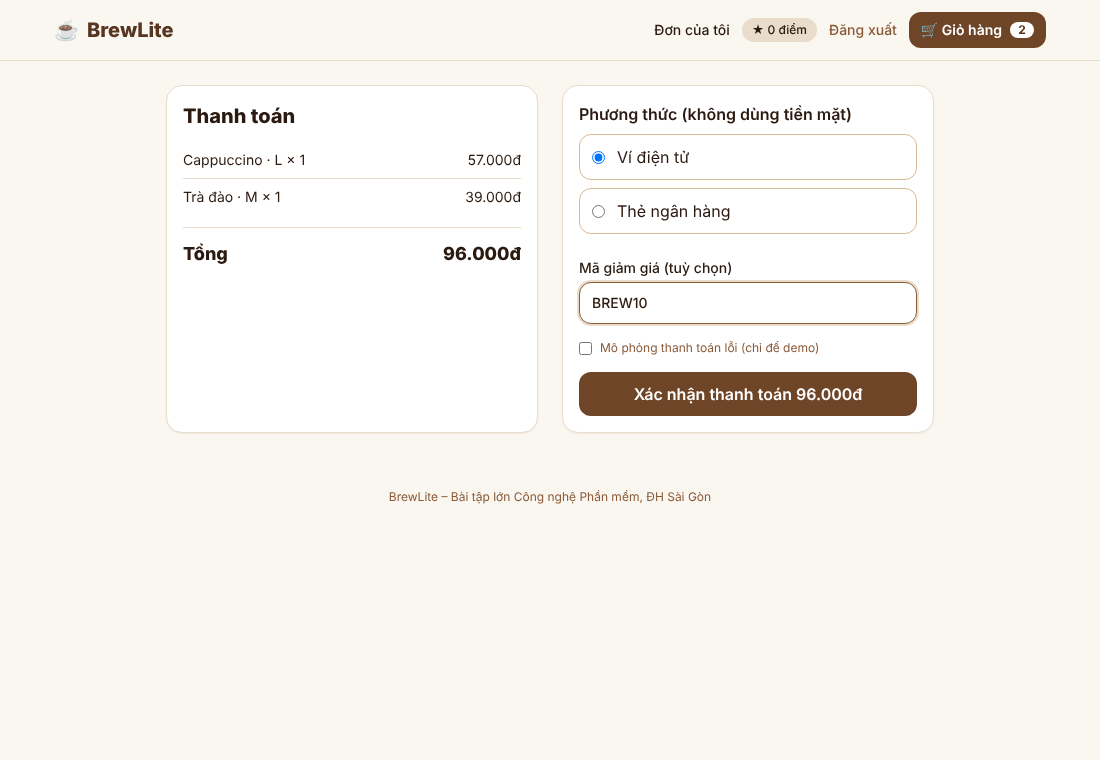
\includegraphics[width=\textwidth]{shots/4-checkout.png}\caption{(4) Thanh toán}\end{subfigure}
\caption{Màn hình Giỏ hàng và Thanh toán}
\end{figure}

\begin{figure}[h!]
\centering
\begin{subfigure}{0.49\textwidth}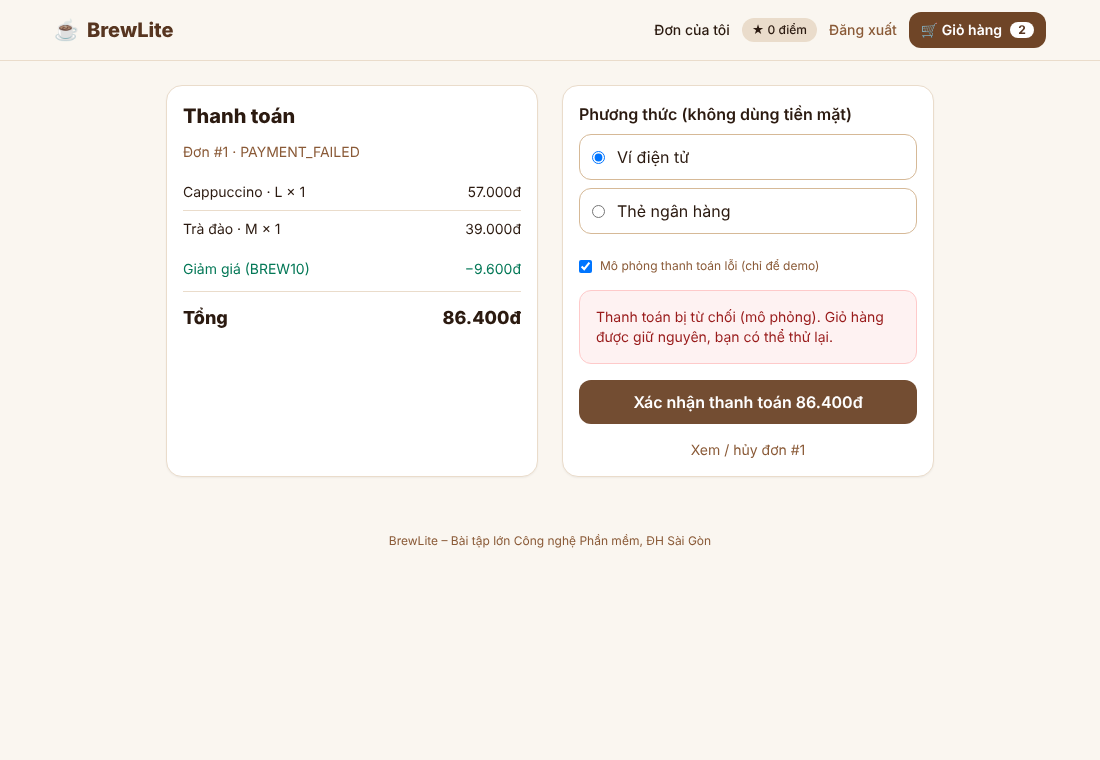
\includegraphics[width=\textwidth]{shots/5-payment-failed.png}\caption{Thanh toán lỗi: giữ giỏ, cho thử lại}\end{subfigure}\hfill
\begin{subfigure}{0.49\textwidth}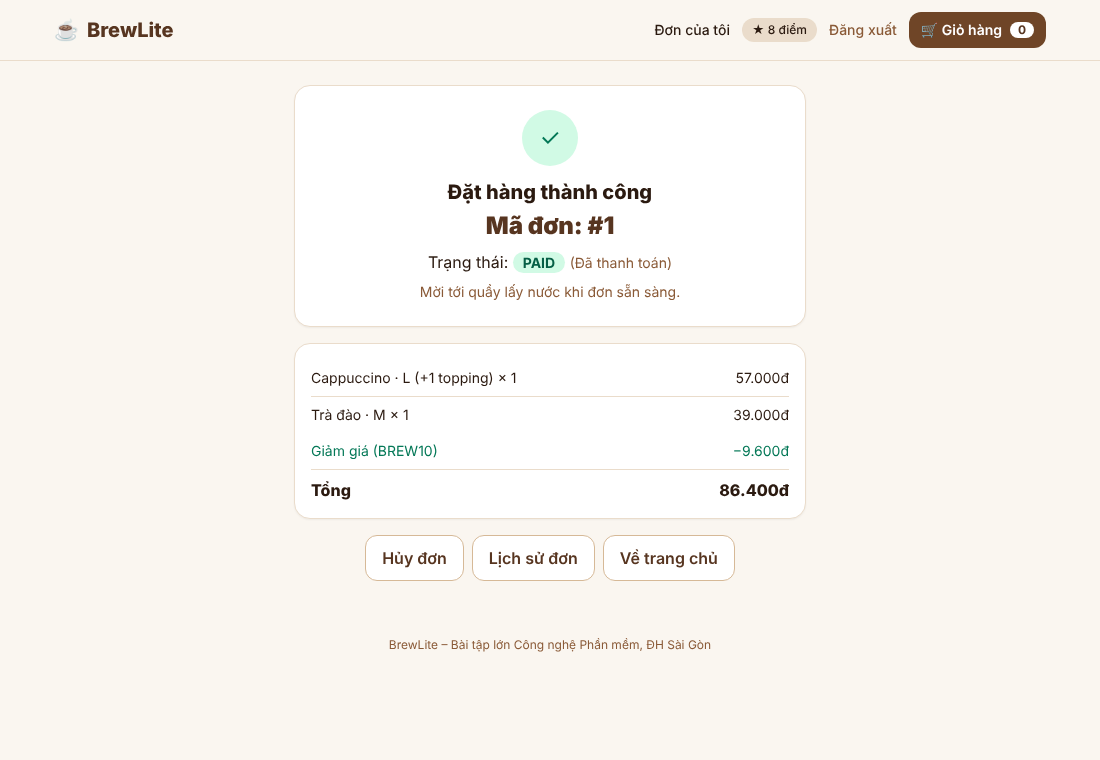
\includegraphics[width=\textwidth]{shots/6-confirmation.png}\caption{(5) Xác nhận đơn thành công}\end{subfigure}
\caption{Luồng thanh toán lỗi và xác nhận}
\end{figure}

\begin{figure}[h!]
\centering
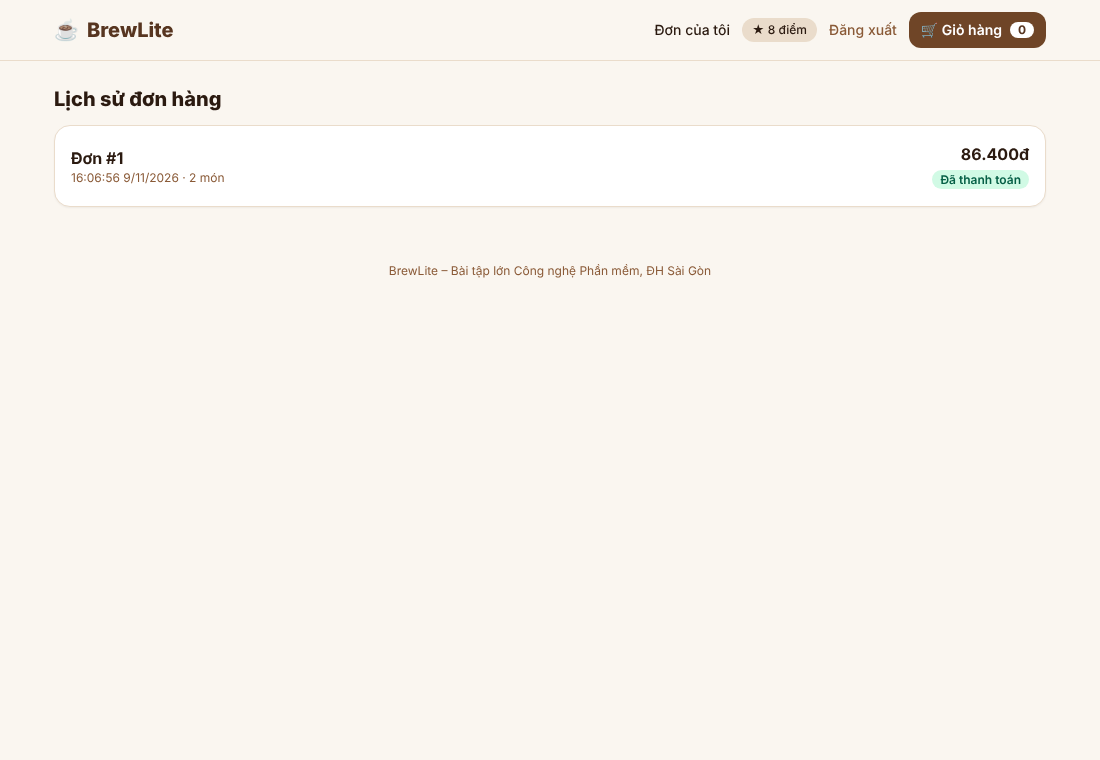
\includegraphics[width=0.6\textwidth]{shots/7-history.png}
\caption{Lịch sử đơn hàng}
\end{figure}

%%%%%%%%%%%%%%%%%%%% 8. BACKLOG %%%%%%%%%%%%%%%%%%%%
\section{Product Backlog: 10 task theo Scrum}\label{sec:backlog}
Mỗi task hoàn thành (đạt Definition of Done ở Mục~\ref{sec:dod}) được 1 điểm, tổng 10 điểm. Cột ``Bằng chứng'' chỉ tới mã nguồn/test trong repository.

\begin{longtable}{|L{0.6cm}|L{2.2cm}|L{3.9cm}|L{0.7cm}|L{0.9cm}|L{3.7cm}|}
\hline
\textbf{\#} & \textbf{Task} & \textbf{Kết quả đạt được} & \textbf{SP} & \textbf{Sprint} & \textbf{Bằng chứng} \\ \hline
\endhead
1 & Khởi tạo dự án và cấu trúc & Monorepo \texttt{backend/} (NestJS) + \texttt{frontend/} (Next.js); chạy được; README, Git, \texttt{.env.example}. & 2 & 1 & \footnotesize \texttt{README.md}, \texttt{backend/.env.example}, \texttt{frontend/.env.example} \\ \hline
2 & API danh sách sản phẩm & \texttt{GET /products} trả JSON (id, tên, giá, ảnh) từ CSDL; kèm \texttt{GET /products/:id}. & 2 & 1 & \footnotesize \texttt{products.controller.ts}; test ``GET /products ...'' \\ \hline
3 & Trang Menu (Frontend) & Gọi \texttt{/products}, hiển thị lưới sản phẩm; có loading, rỗng, lỗi + thử lại. & 3 & 1 & \footnotesize \texttt{frontend/app/page.tsx} \\ \hline
4 & Chi tiết và tuỳ chọn sản phẩm & Chọn size S/M/L và topping; giá tính theo tuỳ chọn; thêm vào giỏ. & 3 & 1 & \footnotesize \texttt{app/products/[id]/page.tsx}; test \texttt{unitPrice} \\ \hline
5 & Giỏ hàng (Cart) & Thêm/sửa số lượng/xóa; state Zustand (lưu \texttt{localStorage}); tự tính tổng tiền; badge số lượng. & 3 & 2 & \footnotesize \texttt{lib/store.ts}, \texttt{app/cart/page.tsx} \\ \hline
6 & API tạo đơn hàng & \texttt{POST /orders} nhận giỏ, validate (class-validator), lưu \st{PENDING}, trả mã đơn. & 3 & 2 & \footnotesize \texttt{orders.service.ts}, \texttt{dto.ts}; test validate đầu vào \\ \hline
7 & Đăng ký / Đăng nhập (JWT) & \texttt{/auth/register}, \texttt{/auth/login}; bcrypt; phát JWT; guard bảo vệ route đặt đơn. & 3 & 2 & \footnotesize \texttt{auth/*}; test ``Task 7'' \\ \hline
8 & Thanh toán không tiền mặt & Mock payment, chọn Ví/Thẻ, \texttt{POST /payments}; \st{PAID} khi thành công, \st{PAYMENT\_FAILED} khi lỗi. & 3 & 3 & \footnotesize \texttt{payments.service.ts}, \texttt{mock-gateway.ts}; test ``Task 8'' \\ \hline
9 & Xác nhận, lịch sử đơn và bàn giao & Màn hình xác nhận (mã đơn, trạng thái), \texttt{GET /orders/me}; docker-compose chạy 3 dịch vụ; README; demo end-to-end. & 3 & 3 & \footnotesize \texttt{app/orders/*}, \texttt{docker-compose.yml}, \texttt{README.md} \\ \hline
10 & Nghiệp vụ backend & State Machine, thanh toán idempotent, tồn kho đồng thời, khuyến mãi/loyalty (Mục~\ref{sec:task10}). & 8 & 3 & \footnotesize \texttt{order-status.ts}, \texttt{stock.service.ts}, \texttt{promotions.service.ts}; 34 test \\ \hline
\multicolumn{3}{|r|}{\textbf{Tổng}} & \textbf{33} & & \textbf{10/10 task hoàn thành} \\ \hline
\caption{Product Backlog và trạng thái hoàn thành}
\end{longtable}

%%%%%%%%%%%%%%%%%%%% 9. TASK 10 %%%%%%%%%%%%%%%%%%%%
\section{Task 10 -- Nghiệp vụ backend: xử lý đặt hàng và thanh toán}\label{sec:task10}
\subsection{Order State Machine}
Luồng thành công: \st{PENDING} \ra{} \st{PAID} \ra{} \st{PREPARING} \ra{} \st{READY} \ra{} \st{COMPLETED}. Ngoại lệ: thanh toán lỗi (\st{PAYMENT\_FAILED}, có thể thử lại về \st{PENDING}) hoặc hủy đơn (\st{CANCELLED}). \st{COMPLETED} và \st{CANCELLED} là trạng thái kết thúc. Mọi chuyển tiếp không có trong sơ đồ bị hàm \texttt{assertTransition} chặn và ném lỗi \texttt{409 INVALID\_TRANSITION}.

\begin{figure}[h!]
\centering
\resizebox{\textwidth}{!}{%
\begin{tikzpicture}[every node/.style={font=\scriptsize\ttfamily},
  s/.style={draw=okgreen,rounded corners,fill=green!8,minimum width=2.1cm,minimum height=8mm,align=center},
  xs/.style={draw=warnred,rounded corners,fill=red!6,minimum width=2.7cm,minimum height=8mm,align=center},
  ok/.style={-{Stealth},thick,okgreen}, ko/.style={-{Stealth},thick,warnred}]
  \node[s] (pe) at (0,0) {PENDING};
  \node[s] (pa) at (3.5,0) {PAID};
  \node[s] (pr) at (7.0,0) {PREPARING};
  \node[s] (re) at (10.5,0) {READY};
  \node[s] (co) at (14.0,0) {COMPLETED};
  \node[xs] (pf) at (0,-3) {PAYMENT\_FAILED};
  \node[xs] (ca) at (5.1,-3) {CANCELLED};
  \draw[-{Stealth},thick] (-1.6,0.9) node[above right] {start} -- (pe.north west);
  \draw[ok] (pe) -- node[above,font=\tiny\sffamily] {thanh toán OK} (pa);
  \draw[ok] (pa) -- node[above,font=\tiny\sffamily] {barista nhận} (pr);
  \draw[ok] (pr) -- node[above,font=\tiny\sffamily] {pha xong} (re);
  \draw[ok] (re) -- node[above,font=\tiny\sffamily] {giao khách} (co);
  \draw[ko] ([xshift=-4mm]pe.south) -- node[left,font=\tiny\sffamily] {thanh toán lỗi} ([xshift=-4mm]pf.north);
  \draw[ko] ([xshift=4mm]pf.north) -- node[right,font=\tiny\sffamily] {thử lại} ([xshift=4mm]pe.south);
  \draw[ko] (pe.south east) -- node[above,sloped,font=\tiny\sffamily,pos=.45] {hủy} (ca.north west);
  \draw[ko] (pf.east) -- node[above,font=\tiny\sffamily] {hủy} (ca.west);
  \draw[ko] (pa.south) -- node[right,font=\tiny\sffamily,pos=.35] {hủy} (ca.north east);
\end{tikzpicture}}
\caption{Sơ đồ máy trạng thái đơn hàng. Đường xanh: luồng thành công; đường đỏ: ngoại lệ}\label{fig:fsm}
\end{figure}

\begin{lstlisting}[caption={Bảng chuyển trạng thái hợp lệ (order-status.ts)}]
export const ORDER_TRANSITIONS = {
  PENDING:        [PAID, PAYMENT_FAILED, CANCELLED],
  PAYMENT_FAILED: [PENDING, CANCELLED],
  PAID:           [PREPARING, CANCELLED],
  PREPARING:      [READY],
  READY:          [COMPLETED],
  COMPLETED:      [],
  CANCELLED:      [],
};
export function assertTransition(from, to) {
  if (!canTransition(from, to)) throw new InvalidOrderTransitionError(from, to);
}
\end{lstlisting}
Để hai yêu cầu đồng thời không cùng chuyển một đơn, bước đổi trạng thái là \texttt{UPDATE orders SET status = :to WHERE id = :id AND status = :from}; nếu không có dòng nào bị ảnh hưởng thì trả \texttt{409}.

\subsection{Thanh toán idempotent}
\texttt{POST /payments} bắt buộc header \texttt{Idempotency-Key}. Thiết kế:
\begin{enumerate}
  \item Cột \texttt{payments.idempotencyKey} có ràng buộc \texttt{UNIQUE}.
  \item Trước khi xử lý, tra cứu theo key: nếu đã có $\Rightarrow$ trả đúng kết quả cũ (HTTP 200, header \texttt{Idempotent-Replayed: true}), không gọi cổng thanh toán, không đổi trạng thái, không cộng điểm lần nữa.
  \item Trong transaction, khóa dòng đơn bằng \texttt{SELECT ... FOR UPDATE}. Các yêu cầu đồng thời trên cùng đơn được xử lý tuần tự; yêu cầu đến sau thấy payment đã tồn tại và trả lại kết quả cũ.
  \item Nếu vẫn xảy ra vi phạm \texttt{UNIQUE} (đua rất sát), bắt lỗi \texttt{23505} và trả kết quả cũ. Dùng lại key cho đơn/người dùng khác $\Rightarrow$ \texttt{409 IDEMPOTENCY\_KEY\_REUSED}.
\end{enumerate}
\texttt{POST /orders} cũng nhận \texttt{Idempotency-Key} (ràng buộc \texttt{UNIQUE(userId, idempotencyKey)}), nên gửi lặp cùng key chỉ tạo 1 đơn và trừ kho 1 lần.

\subsection{Kiểm soát tồn kho khi đặt đồng thời}
Khi tạo đơn, kho được giữ trong cùng transaction với việc lưu đơn. Mỗi lần trừ kho dùng \textbf{optimistic locking} với cột \texttt{version}: câu lệnh chỉ cập nhật nếu \texttt{version} chưa đổi; nếu giao dịch khác đã thắng thì đọc lại và thử lại (tối đa 8 lần). Thiếu hàng $\Rightarrow$ \texttt{409 OUT\_OF\_STOCK} và rollback toàn bộ đơn (không trừ kho các sản phẩm khác). Các sản phẩm được trừ theo thứ tự \texttt{id} để tránh deadlock; hủy đơn hoàn kho.

\begin{lstlisting}[caption={Giữ kho bằng optimistic locking (stock.service.ts, rút gọn)}]
for (let attempt = 0; attempt < MAX_RETRIES; attempt++) {
  const p = await m.findOne(Product, { where: { id } });
  if (p.stock < qty) throw new ConflictException(OUT_OF_STOCK);
  const res = await m.update(Product,
      { id, version: p.version },                 // chi thanh cong neu version chua doi
      { stock: p.stock - qty, version: p.version + 1 });
  if (res.affected === 1) return;                 // thang -> xong
  // thua: giao dich khac da doi version -> doc lai va thu lai
}
throw new ConflictException(CONTENTION);
\end{lstlisting}

\subsection{Khuyến mãi và điểm thưởng}
Mã giảm giá được kiểm tra: tồn tại, còn hoạt động, chưa hết hạn, đạt đơn tối thiểu; số tiền giảm = phần trăm $\times$ tạm tính (làm tròn xuống), không vượt trần \texttt{maxDiscount}. Điểm thưởng: 1 điểm cho mỗi 10.000đ của đơn, chỉ cộng khi đơn chuyển \st{PAID} và đúng một lần (cờ \texttt{pointsAwarded} cập nhật có điều kiện). Mã mẫu: \texttt{BREW10} (10\%, tối đa 20.000đ) và \texttt{WELCOME20} (20\% cho đơn từ 100.000đ, tối đa 50.000đ).

%%%%%%%%%%%%%%%%%%%% 10. KIỂM THỬ %%%%%%%%%%%%%%%%%%%%
\section{Kết quả kiểm thử}\label{sec:test}
Chạy bằng \texttt{npm run test:all} trong \texttt{backend/} (PostgreSQL 16 thật, schema được tạo mới mỗi lần): \textbf{3 test suite, 34 test, tất cả đạt}; chạy lặp 3 lần liên tiếp đều ổn định.

\subsection{Ba tiêu chí chấm của Task 10}
\begin{table}[h!]
\centering
\begin{tabularx}{\textwidth}{|L{2.6cm}|X|L{3.2cm}|}
\hline
\textbf{Tiêu chí} & \textbf{Test chứng minh} & \textbf{Kết quả} \\ \hline
(a) Chặn chuyển trạng thái sai & Unit: kiểm tra toàn bộ 49 cặp (từ, đến); đúng 9 cặp được phép, 40 cặp còn lại bị chặn. Integration: \st{PENDING}\ra\st{READY}, \st{PAID}\ra\st{READY}, \st{COMPLETED}\ra\st{PREPARING} đều trả 409 \texttt{INVALID\_TRANSITION}; luồng đúng đi hết \st{COMPLETED}. & Đạt \\ \hline
(b) Cùng Idempotency-Key chỉ tạo 1 đơn & Gửi 2 lần tuần tự (lần 2 trả 200, cùng \texttt{id}, kho chỉ trừ 1 lần); 5 yêu cầu \textbf{đồng thời} cùng key chỉ tạo 1 đơn; 4 yêu cầu thanh toán đồng thời cùng key chỉ có 1 giao dịch (1 lần 201), điểm thưởng cộng đúng 1 lần (13 điểm cho đơn 135.000đ). & Đạt \\ \hline
(c) Đặt đồng thời không vượt tồn kho & 12 khách đặt cùng lúc 1 sản phẩm còn 5: đúng 5 đơn \texttt{201}, 7 đơn \texttt{409 OUT\_OF\_STOCK}, kho về 0 (không âm), tổng số lượng bán = 5. Kho 7, 6 khách mua 2 ly: đúng 3 đơn thành công, còn 1. & Đạt \\ \hline
\end{tabularx}
\caption{Đối chiếu tiêu chí chấm Task 10 với test}
\end{table}

\subsection{Danh sách test}
\begin{longtable}{|L{3.6cm}|L{8.4cm}|L{1.3cm}|}
\hline
\textbf{Nhóm} & \textbf{Nội dung kiểm tra} & \textbf{Kết quả} \\ \hline
\endhead
Unit -- State machine (4) & Cho phép đúng chuyển tiếp hợp lệ; chặn 40/49 cặp còn lại; trạng thái kết thúc; không nhảy cóc. & 4/4 đạt \\ \hline
Unit -- Tính giá (3) & Chênh lệch size; cộng topping, bỏ trùng; lỗi với size/topping sai. & 3/3 đạt \\ \hline
Unit -- Khuyến mãi (4) & Giảm phần trăm làm tròn xuống; trần giảm giá; từ chối mã sai/hết hạn/chưa đủ đơn tối thiểu; quy đổi điểm. & 4/4 đạt \\ \hline
Task 2 -- Sản phẩm (1) & Danh sách (id, tên, giá, ảnh), chi tiết kèm tuỳ chọn, 404. & 1/1 đạt \\ \hline
Task 7 -- Xác thực (3) & Đăng ký/đăng nhập, bcrypt, \texttt{/auth/me}; email trùng 409, sai mật khẩu 401, dữ liệu sai 400; guard 401. & 3/3 đạt \\ \hline
Task 6 -- Tạo đơn (3) & Server tự tính giá, trừ kho; validate (giỏ rỗng, size sai, số lượng sai, trường lạ, sản phẩm không có); chỉ xem đơn của mình. & 3/3 đạt \\ \hline
Task 8 -- Thanh toán (3) & Thành công $\to$ \st{PAID}; thiếu key 400; lỗi 402 $\to$ \st{PAYMENT\_FAILED} rồi thử lại $\to$ \st{PAID}; không thanh toán lại đơn đã PAID; không thanh toán đơn người khác. & 3/3 đạt \\ \hline
Task 10.1 -- State machine (3) & Chặn chuyển sai qua API; phân quyền nhân viên; hủy đơn hoàn kho. & 3/3 đạt \\ \hline
Task 10.2 -- Idempotent (4) & Đơn lặp tuần tự và đồng thời; thanh toán lặp/đồng thời; dùng key cho đơn khác 409. & 4/4 đạt \\ \hline
Task 10.3 -- Tồn kho (3) & 12 khách tranh 5 sản phẩm; mua nhiều số lượng; rollback khi thiếu giữa chừng. & 3/3 đạt \\ \hline
Task 10.4 -- Khuyến mãi (3) & Áp mã, cộng điểm chỉ khi PAID, thu hồi điểm khi hủy đơn đã thanh toán; từ chối mã không hợp lệ. & 3/3 đạt \\ \hline
\multicolumn{2}{|r|}{\textbf{Tổng}} & \textbf{34/34 đạt} \\ \hline
\caption{Tổng hợp 34 test tự động}
\end{longtable}

\subsection{Kiểm thử giao diện end-to-end}
Kịch bản Playwright (Chromium) trên bản build production: mở Menu (8 sản phẩm) $\to$ chọn Cappuccino size L + trân châu (giá hiển thị 57.000đ) $\to$ thêm giỏ $\to$ thêm Trà đào (size M) $\to$ giỏ (2 dòng, tổng 96.000đ) $\to$ bấm Thanh toán khi chưa đăng nhập (chuyển \texttt{/login}) $\to$ đăng ký $\to$ thanh toán \textbf{lỗi} có mã \texttt{BREW10} (đơn \st{PAYMENT\_FAILED}, giỏ còn 2 dòng) $\to$ thử lại thành công $\to$ màn hình xác nhận (mã đơn \#1, \st{PAID}, tổng 86.400đ sau giảm 9.600đ, cộng 8 điểm, giỏ rỗng) $\to$ lịch sử đơn (1 đơn). Không có lỗi JavaScript ngoài phản hồi 402 có chủ đích.

\subsection{Kiểm thử giao diện mở rộng và lỗi nghiệp vụ phát hiện}\label{sec:uitest}
Ngoài kịch bản chính ở trên, một bộ \textbf{55 kịch bản} Playwright (Chromium thật, backend và PostgreSQL thật) được chạy để tìm lỗi \emph{nghiệp vụ}. Sau mỗi thao tác trên giao diện, kịch bản đối chiếu lại cơ sở dữ liệu (số đơn, trạng thái, tồn kho, điểm thưởng, số giao dịch thanh toán). Các tình huống bất thường được mô phỏng: ngắt mạng đúng lúc nhận phản hồi, bấm liên tục, hai trình duyệt cùng mua ly cuối, giá đổi khi khách đang xem giỏ, token hỏng, tải lại giữa chừng. Kết quả lượt chạy cuối (sau khi sửa lỗi): \textbf{55/55 kịch bản, 224/224 điểm kiểm tra đạt}.

\begin{table}[h!]
\centering
\begin{tabularx}{\textwidth}{|X|c|c|c|}
\hline
\textbf{Nhóm kiểm thử} & \textbf{Kịch bản} & \textbf{Điểm kiểm tra} & \textbf{Kết quả} \\ \hline
A. Menu và chi tiết sản phẩm & 8 & 25 & 8/8 \\ \hline
B. Giỏ hàng & 5 & 16 & 5/5 \\ \hline
C. Tài khoản và phân quyền giao diện & 9 & 21 & 9/9 \\ \hline
D. Thanh toán và mã giảm giá & 12 & 56 & 12/12 \\ \hline
E. Đơn hàng: lịch sử, chi tiết, hủy, trạng thái & 6 & 21 & 6/6 \\ \hline
F. Tồn kho và dữ liệu thay đổi & 5 & 20 & 5/5 \\ \hline
G. Bảo mật và kiểm tra dữ liệu đầu vào (API) & 7 & 55 & 7/7 \\ \hline
H. Giao diện di động và độ ổn định & 3 & 10 & 3/3 \\ \hline
\textbf{Tổng} & \textbf{55} & \textbf{224} & \textbf{55/55} \\ \hline
\end{tabularx}
\caption{Tổng hợp kiểm thử giao diện theo nhóm}
\end{table}

Lượt chạy đầu tiên phát hiện 6 lỗi, đã sửa và chạy lại toàn bộ (chi tiết từng kịch bản, ảnh chụp: \texttt{docs/BrewLite\_Bao\_cao\_kiem\_thu.pdf}):
\begin{longtable}{|L{0.9cm}|L{1.3cm}|L{4.2cm}|L{5.8cm}|}
\hline
\textbf{Mã} & \textbf{Mức} & \textbf{Lỗi} & \textbf{Cách sửa} \\ \hline
\endhead
F04 & Cao & Giá server đổi sau khi khách bỏ món vào giỏ nhưng vẫn thanh toán: khách bị trừ số tiền chưa được thấy. & Thanh toán so sánh tổng đơn với tổng giỏ; lệch thì dừng, báo giá mới và chờ khách xác nhận lại. \\ \hline
D11 & Trung bình & Thanh toán lỗi rồi tải lại trang tạo đơn thứ hai; đơn lỗi cũ vẫn giữ kho. & Khi lỗi, đưa về \texttt{/checkout?order=ID} để thử lại dùng đúng đơn cũ. \\ \hline
D12 & Trung bình & Thanh toán lại từ trang chi tiết đơn xong nhưng giỏ không được xóa. & Chỉ xóa các dòng giỏ khớp món trong đơn đã thanh toán. \\ \hline
E06 & Trung bình & Hủy đơn đã thanh toán không thu hồi điểm thưởng (mua rồi hủy vẫn giữ điểm). & Thêm \texttt{revokePoints} dùng cờ \texttt{pointsAwarded} (hủy hai lần không trừ hai lần) và test tích hợp. \\ \hline
C07 & Thấp & Token hết hạn hoặc hỏng: giao diện kẹt ở trạng thái đã đăng nhập, lỗi lặp lại. & Nhận 401 thì tự đăng xuất và chuyển về \texttt{/login}. \\ \hline
G07 & Thấp & Không đặt \texttt{CORS\_ORIGIN} thì chấp nhận mọi nguồn gốc. & Mặc định chỉ cho phép \texttt{http://localhost:3000}. \\ \hline
\caption{Lỗi nghiệp vụ phát hiện qua kiểm thử giao diện}
\end{longtable}

\subsection{Hạn chế đã biết}
{\sloppy Các điểm sau nằm ngoài yêu cầu của đề, được ghi rõ để tránh hiểu nhầm là đã làm: (1) đơn \st{PENDING} không tự hết hạn nên có thể giữ kho vô thời hạn; (2) giỏ hàng lưu theo trình duyệt, không theo tài khoản; (3) cổng thanh toán là giả lập và chưa có quy trình hoàn tiền khi hủy đơn đã thanh toán; (4) tồn kho tính theo sản phẩm, không theo nguyên liệu; (5) chưa có giao diện cho nhân viên (cập nhật trạng thái qua API); (6) JWT lưu trong \texttt{localStorage}; (7) mới kiểm thử trên Chromium, chưa kiểm thử tải lớn.\par}

%%%%%%%%%%%%%%%%%%%% 11. DoD %%%%%%%%%%%%%%%%%%%% 
\section{Definition of Done}\label{sec:dod}
\begin{table}[h!]
\centering
\begin{tabularx}{\textwidth}{|X|L{6.6cm}|}
\hline
\textbf{Tiêu chí DoD} & \textbf{Minh chứng} \\ \hline
Code chạy được, không lỗi build; đúng tiêu chí chấp nhận & \texttt{npm run build} (backend) và \texttt{next build} (frontend) thành công; 34 test đạt \\ \hline
Có commit Git với mô tả rõ ràng; được review trong nhóm & Lịch sử Git của repository (commit theo thành phần/task); do dự án một thành viên nên tự review theo checklist DoD trước mỗi lần commit/merge \\ \hline
API có validate đầu vào; UI xử lý loading/lỗi cơ bản & \texttt{ValidationPipe} + DTO; test 400; Spinner/ErrorBox/Empty ở mọi trang tải dữ liệu \\ \hline
Có hướng dẫn chạy trong README & \texttt{README.md}: chạy bằng Docker Compose, chạy thủ công, kiểm thử, API, tài khoản mẫu \\ \hline
\end{tabularx}
\caption{Đối chiếu Definition of Done}
\end{table}

%%%%%%%%%%%%%%%%%%%% 12. BÀN GIAO %%%%%%%%%%%%%%%%%%%%
\section{Bàn giao sản phẩm cho khách hàng}\label{sec:handover}
\subsection{Kịch bản Sprint Review / Demo}
\begin{enumerate}
  \item Chạy \texttt{docker compose up --build}; mở \texttt{http://localhost:3000}.
  \item Trình diễn luồng end-to-end: chọn sản phẩm $\to$ giỏ hàng $\to$ đăng ký/đăng nhập $\to$ thanh toán $\to$ xác nhận đơn.
  \item Demo nhánh lỗi: bật ``Mô phỏng thanh toán lỗi'' $\to$ đơn \st{PAYMENT\_FAILED}, giỏ giữ nguyên $\to$ thử lại thành công.
  \item Demo mã giảm giá \texttt{BREW10} và điểm thưởng ở thanh tiêu đề.
  \item Chạy \texttt{npm run test:all} để chứng minh ba tiêu chí Task 10.
  \item (Mở rộng) dùng tài khoản nhân viên \texttt{staff@brewlite.local} gọi \texttt{PATCH /orders/:id/status} để chuyển \st{PREPARING} $\to$ \st{READY} $\to$ \st{COMPLETED}; trang xác nhận tự cập nhật.
\end{enumerate}

\subsection{Danh mục bàn giao}
Mã nguồn Git (\texttt{backend/}, \texttt{frontend/}), \texttt{docker-compose.yml} chạy được cả 3 dịch vụ, \texttt{README.md}, \texttt{.env.example}, báo cáo này, báo cáo kiểm thử giao diện, bộ kịch bản Playwright, ảnh chụp màn hình, các sơ đồ dạng draw.io (\texttt{docs/drawio/}, chỉnh sửa được) và kết quả test trong \texttt{docs/}.

\subsection{Sprint Retrospective}
Retrospective được thực hiện vào cuối Sprint 3 (10/11/2026) với cách nhìn lại cả ba Sprint.
\begin{tabularx}{\textwidth}{|X|X|}
\hline
\textbf{Điều làm tốt} & \textbf{Điều cần cải thiện} \\ \hline
\begin{itemize}\itemsep0pt
  \item Kiểm thử giao diện có đối chiếu cơ sở dữ liệu tìm ra 6 lỗi nghiệp vụ mà test API không thấy (ví dụ giá đổi khi khách đang xem giỏ).
  \item Viết test song song với nghiệp vụ khó (đồng thời, idempotent) nên phát hiện sớm lỗi đua dữ liệu.
  \item Server luôn tính lại giá, client không thể gian lận giá.
  \item Tách hàm thuần (giá, giảm giá, state machine) giúp unit test nhanh.
  \item Docker Compose giúp chạy lại toàn hệ thống bằng một lệnh.
\end{itemize} &
\begin{itemize}\itemsep0pt
  \item Dùng \texttt{synchronize} của TypeORM cho tiện demo; sản phẩm thật cần migration.
  \item Chưa có xác thực thanh toán thật và webhook; hiện dùng cổng giả lập.
  \item Chưa có test tự động cho giao diện trong CI (mới có kịch bản Playwright chạy tay).
  \item Cập nhật Burndown hằng ngày cần kỷ luật hơn trong Daily Scrum.
\end{itemize} \\ \hline
\end{tabularx}

\subsection{Phản hồi của ``khách hàng'' và backlog cho phiên bản sau}
Tại buổi Sprint Review, Product Owner nhận xét: luồng đặt hàng end-to-end chạy đúng, giá luôn do server tính, nhánh thanh toán lỗi giữ lại giỏ hàng là hợp lý; đồng thời đề nghị bổ sung giao diện cho nhân viên quầy và thanh toán thật ở phiên bản sau. % TODO-EDIT: thay bằng phản hồi thực tế sau buổi demo
Các hạng mục đề xuất cho phiên bản 1.1:
\begin{itemize}
  \item Giao diện nhân viên quầy/barista (hàng đợi đơn, cập nhật trạng thái).
  \item Tích hợp cổng thanh toán thật (VNPay/Momo/Stripe) và webhook xác nhận.
  \item Thông báo thời gian thực (WebSocket/SSE) khi đơn \st{READY}.
  \item Migration CSDL, giới hạn tần suất (rate limit), refresh token.
  \item Quản trị menu, tồn kho theo nguyên liệu, báo cáo doanh thu.
\end{itemize}

%%%%%%%%%%%%%%%%%%%% 13. API %%%%%%%%%%%%%%%%%%%%
\section{API và chức năng tối thiểu}
\subsection{Các endpoint}
\begin{table}[h!]
\centering\small
\begin{tabularx}{\textwidth}{|L{4.1cm}|X|L{1.8cm}|}
\hline
\textbf{Endpoint} & \textbf{Chức năng} & \textbf{Xác thực} \\ \hline
\texttt{GET /products} & Danh sách sản phẩm (menu) & --- \\ \hline
\texttt{GET /products/:id} & Chi tiết một sản phẩm + tuỳ chọn size/topping & --- \\ \hline
\texttt{POST /auth/register} & Đăng ký tài khoản, trả JWT & --- \\ \hline
\texttt{POST /auth/login} & Đăng nhập, trả JWT & --- \\ \hline
\texttt{GET /auth/me} & Thông tin tài khoản, điểm thưởng & JWT \\ \hline
\texttt{POST /orders} & Tạo đơn (\st{PENDING}); hỗ trợ \texttt{Idempotency-Key} & JWT \\ \hline
\texttt{POST /payments} & Thanh toán (idempotent). 201 thành công, 200 phát lại, 402 lỗi & JWT \\ \hline
\texttt{GET /orders/me} & Lịch sử đơn của người dùng & JWT \\ \hline
\texttt{GET /orders/:id} & Chi tiết một đơn (chủ đơn hoặc nhân viên) & JWT \\ \hline
\texttt{POST /orders/:id/cancel} & Hủy đơn, hoàn kho & JWT \\ \hline
\texttt{PATCH /orders/:id/status} & Nhân viên chuyển trạng thái pha chế (mở rộng) & JWT, STAFF \\ \hline
\end{tabularx}
\caption{Các endpoint của backend}
\end{table}

\subsection{Thực thể tối thiểu}
\begin{itemize}
  \item \texttt{Product(id, name, price, imageUrl, stock)} --- thêm \texttt{description}, \texttt{version} (optimistic locking).
  \item \texttt{User(id, email, passwordHash, loyaltyPoints)} --- thêm \texttt{name}, \texttt{role}.
  \item \texttt{Order(id, userId, status, total, createdAt)} --- thêm \texttt{subtotal},\allowbreak{} \texttt{discount},\allowbreak{} \texttt{couponCode},\allowbreak{} \texttt{idempotencyKey},\allowbreak{} \texttt{pointsAwarded}.
  \item \texttt{OrderItem(id, orderId, productId, size, qty, lineTotal)} --- thêm \texttt{productName}, \texttt{toppings}, \texttt{unitPrice}.
  \item \texttt{Payment(id, orderId, idempotencyKey, amount, method)} --- thêm \texttt{userId}, \texttt{status}, \texttt{reference}, \texttt{failureReason}.
\end{itemize}

%%%%%%%%%%%%%%%%%%%% 14. KẾT LUẬN %%%%%%%%%%%%%%%%%%%%
\section{Kết luận}
Nhóm đã xây dựng BrewLite theo Agile Scrum, hoàn thành 10/10 task: từ khởi tạo dự án, menu, giỏ hàng, đăng nhập JWT, đặt đơn, thanh toán không tiền mặt, đến các nghiệp vụ backend thực tế (state machine, idempotent, tồn kho đồng thời, khuyến mãi/điểm thưởng) có test chứng minh. Kiểm thử giao diện (55 kịch bản) tìm và giúp sửa thêm 6 lỗi nghiệp vụ. Hạn chế hiện tại là cổng thanh toán giả lập, chưa có giao diện barista và chưa dùng migration (xem thêm Mục~\ref{sec:uitest}); các hạng mục này được ghi vào backlog cho phiên bản tiếp theo.

%%%%%%%%%%%%%%%%%%%% TÀI LIỆU THAM KHẢO %%%%%%%%%%%%%%%%%%%%
\begin{thebibliography}{80}
\bibitem{scrum} K. Schwaber, J. Sutherland, ``\textbf{The Scrum Guide}'', \textit{scrumguides.org}, 2020. \url{https://scrumguides.org/scrum-guide.html}
\bibitem{nest} NestJS, ``\textbf{NestJS Documentation}'', \url{https://docs.nestjs.com/}
\bibitem{next} Vercel, ``\textbf{Next.js Documentation}'', \url{https://nextjs.org/docs}
\bibitem{typeorm} TypeORM, ``\textbf{Transactions, Optimistic/Pessimistic Locking}'', \url{https://typeorm.io/}
\bibitem{pg} PostgreSQL Global Development Group, ``\textbf{Explicit Locking (SELECT ... FOR UPDATE)}'', \url{https://www.postgresql.org/docs/16/explicit-locking.html}
\bibitem{idem} IETF, ``\textbf{The Idempotency-Key HTTP Header Field}'' (draft), \url{https://datatracker.ietf.org/doc/draft-ietf-httpapi-idempotency-key-header/}
\end{thebibliography}
\end{document}
